\documentclass{VUMIFPSkursinis}
\usepackage{algorithmicx}
\usepackage{algorithm}
\usepackage{algpseudocode}
\usepackage{amsfonts}
\usepackage{amsmath}
\usepackage{booktabs}
\usepackage{blindtext}
\usepackage{bm}
\usepackage{caption}
\usepackage{color}
\usepackage{colortbl}
\usepackage{float}
\usepackage{graphicx}
\usepackage{listings}
\usepackage{multirow}
\usepackage{scrextend}
\usepackage{subfig}
\usepackage{wrapfig}
\usepackage{longtable}
\usepackage{enumitem}
\usepackage{xparse}
%\usepackage{tabularx}
\usepackage{ltxtable}
\usepackage{tabu}
\usepackage{xcolor}

% Titulinio aprašas
\university{Vilniaus universitetas}
\faculty{Matematikos ir informatikos fakultetas}
\department{Programų sistemų katedra}
\papertype{3 laboratorinis darbas}
\title{Lietuvos Nacionalinė Sporto Organizacija }
\titleineng{Lithuanian National Sports Organization}
\status{2 kurso 5 grupės studentai}
\author{Margiris Strakšys}
\secondauthor{Gabrielė Saletytė}
\thirdauthor{Vytautas Strimaitis}
\fourthauthor{Gabijus Arūnas Šukaitis}
\supervisor{lekt. Vytautas Valaitis}
\date{Vilnius – \the\year}

% Nustatymai
% \setmainfont{Palemonas}   % Pakeisti teksto šriftą į Palemonas (turi būti įdiegtas sistemoje)
%\bibliography{bibliografija}

%==========================================================================> Dokumento pradžia <========================================================================
\begin{document}
    \maketitle
    \tableofcontents
	
    \sectionnonum{Anotacija} \label{anotacija}
        Šiuo darbu siekiama, apibrėžti programų sistemos eskizinį projektą.
		Šiame laboratoriniame darbe bus analizuojami programų sistemos projektiniai reikalavimai, jų pakirtis, struktūra, ir turinys.
		Darbas atliekamas, pasinaudojant 4+1 architektūros pjūvių modelį, naudojamą apibrėžti ir specifikuoti kuriamą programų sistemą.
		
    \sectionnonum{Įvadas} \label{ivadas}
        \subsection*{Programų sistemos pavadinimas} \label{ivadas_pavadinimas}
			„Lietuvos nacionalinė sporto organizcija” (sutrumpintas sistemos pavadinimas - „LtNSO”).

		\subsection*{Darbo tikslas} \label{ivadas_tikslas}
			Pagal architektūrinio pjūvio modelį, apibrėžti ir specifikuoti: užduotis ir jų vykdymo scenarijus, struktūrinį ir dinaminį programų sistemos modelius, programų sistemos komponentus ir jų skirstymą tinkle.
		
		\subsection*{Temos aktualumas} \label{ivadas_aktualumas}
			Lietuvos nacionalinės sporto organizacijos internetinis puslapis yra projektas, skirtas populiarinti sportą Lietuvoje, skatinti lietuvių sportiškumą ir tuo pačiu gerinti visuomenės sveikatą.
			Plėtoti lietuvių tautinį identitetą, žaidžiant už savo miestą ar rajoną. 
			Tinklapis, kartu su sistema, yra patraukli vieta skelbti reklamą Lietuvos verslui. 
			Sportas ir aktyvus laisvalaikis yra populiarus visuomenėje, todėl puslapis pritrauks daug žmonių.
		
		\subsection*{Naudotojai} \label{ivadas_naudotojai}
			Informacinė sistema skirta organizatoriams, komitetui, dalyviams, darbuotojams bei visiems susidomėjusiems.

		\subsection*{Darbo pagrindas}  \label{ivadas_darboPagrindas}
			Dokumentas parengtas kaip programų sistemų inžinerijos laboratorinis darbas.
			
    \section{Užduotys ir jų vykdymo scenarijai} \label{uzduotysIrJuVykdymoScenarijai}
	
        \subsubsection*{Renginio organizavimas}
		
			\begin{figure}[H]
				\centering
				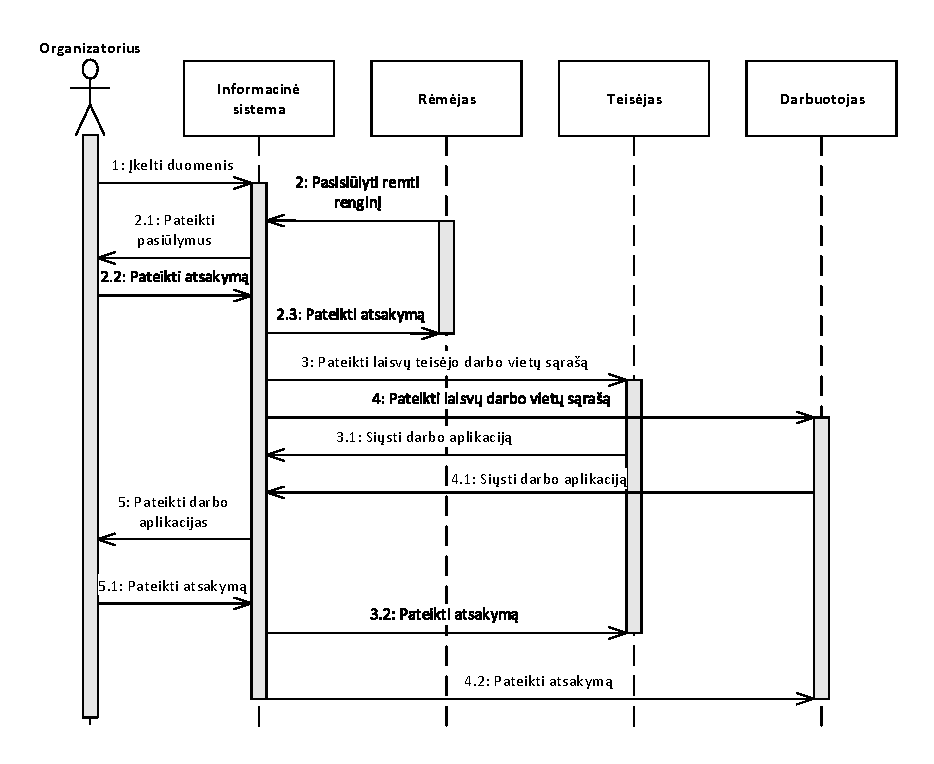
\includegraphics[width=\textwidth]{img/IsPSI1ScenarijausSekuDiagrama1}
				\caption{Renginio organizavimo UML sekų diagrama}
				\label{fig:scenarijusOrganizavimoSekuDiagrama}
			\end{figure}

			\begin{enumerate}
				\item \underline{Organizatorius} į \underline{informacinę sistemą} \textit{įkelia renginio duomenis} - galimas sporto šakas, tvarkaraščius, laisvų vietų skaičių, kiekvienos sporto šakos varžybų vietą ir t.t. 
				\item \underline{Rėmėjas} \underline{informacinėje sistemoje} \textit{pasisiūlo remti renginį}. 
				\begin{itemize}
					\item \underline{Informacinėje sistemoje} esantys \underline{rėmėjų} pasiūlymai yra \textit{pateikiami} \underline{organizatoriui}.
					\item \underline{Organizatorius}, apsvarstęs pateiktą rėmėjo pasiūlymą, \textit{pateikia atsakymą}, t.y. paramos pasiūlymą priima arba atmeta, \underline{informacinėje sistemoje}.
					\item \underline{Informacinėje sistemoje} yra \textit{pateikiamas \underline{organizatoriaus} atsakymas}, kurį gali peržiūrėti \underline{rėmėjas}.
				\end{itemize}
				\item \underline{Informacinėje sistemoje} \textit{pateikiamas laisvų teisėjo darbo vietų sąrašas}, kurį potencialus \underline{teisėjas} gali peržvelgti.
				\begin{itemize}
					\item Potencialus \underline{teisėjas} \textit{siunčia darbo aplikaciją} į \underline{informacinę sistemą}.
					\item \underline{Teisėjas} peržiūri \underline{informacinėje sistemoje} \textit{pateiktą atsakymą}.
				\end{itemize}
				\item \underline{Informacinėje sistemoje} \textit{pateikiamas laisvų darbo vietų sąrašas}, kurį gali peržiūrėti potencialus \underline{darbuotojas}.
				\begin{itemize}
					\item Potencialus \underline{darbuotojas} \textit{siunčia darbo aplikaciją} į \underline{informacinę sistemą}.
					\item \underline{Darbuotojas} peržiūri \underline{informacinėje sistemoje} \textit{pateiktą atsakymą}.
				\end{itemize}
				\item \underline{Organizatorius} peržiūri \underline{informacinėje sistemoje} \textit{pateiktas darbo aplikacijas}.
				\begin{itemize}
					\item \underline{Organizatorius}, apsvarstęs darbo aplikacijas, išsirenka geriausius kandidatus ir jų aplikacijas patvirtina, o kitas atmeta. Tada \textit{pateikia atsakymą}  \underline{informacinėje sistemoje}.
				\end{itemize}
			\end{enumerate}

    \subsubsection*{Dalyvavimas renginyje}
	
	    \begin{figure}[H]
			\centering
			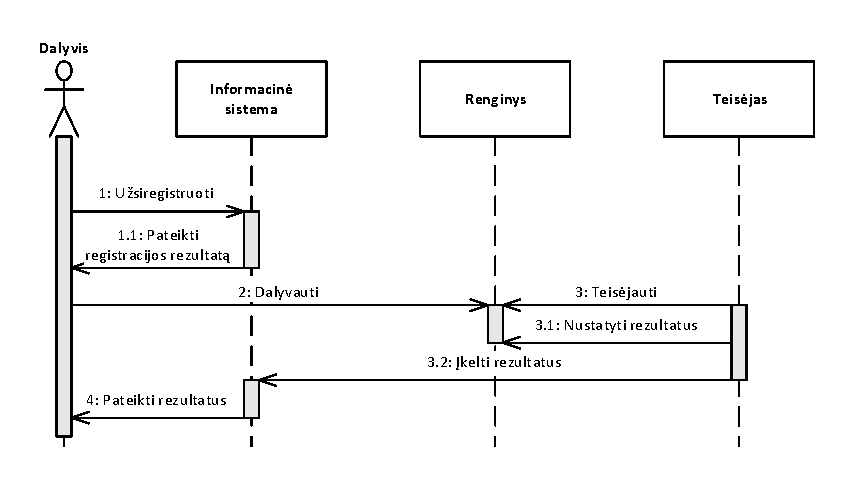
\includegraphics[width=\textwidth]{img/IsPSI1ScenarijausSekuDiagrama2}
			\caption{Dalyvavimo renginyje UML sekų diagrama}
			\label{fig:scenarijusDalyvavimoSekuDiagrama}
		\end{figure}
      
		\begin{enumerate}
			\item  \underline{Dalyvis}, pasirinkęs rungtį, kurioje nori dalyvauti, \textit{užsiregiztruoja} \underline{informacinėje sistemoje}.
			\begin{itemize}
				\item \underline{Dalyvis} peržiūri \underline{informacinėje sistemoje}  \textit{pateiktą registracijos rezultatą}. Jis gali būti tiek teigiamas, kai
					registracija buvo sėkminga, tiek neigiamas, jei įvyko kažkokia klaida (pavyzdžiui, nebeliko laisvų vietų).
			\end{itemize}
			\item \underline{Dalyvis} \textit{dalyvauja} \underline{renginyje} ir varžosi dėl prizinių vietų.
			\item \underline{Teisėjas} \textit{teisėjauja} \underline{renginyje}. Jam padeda kiti darbuotojai, kurie rūpinasi, kad \underline{renginys} vyktų sklandžiai. 
			\begin{itemize}
				\item \underline{Teisėjas} \underline{renginio} metu fiksuoja bei  \textit{nustato rezultatus}.
				\item  \underline{Teisėjo} fiksuoti  \textit{rezultatai įkeliami} į \underline{informacinę sistemą}.
			\end{itemize}
			\item \underline{Dalyvis} gali peržiūrėti \underline{informacinėje sistemoje}  \textit{pateiktus rezultatus}. 
		\end{enumerate}
      
    \subsubsection*{Naujo pasiūlymo teikimas}
	
	    \begin{figure}[H]
			\centering
			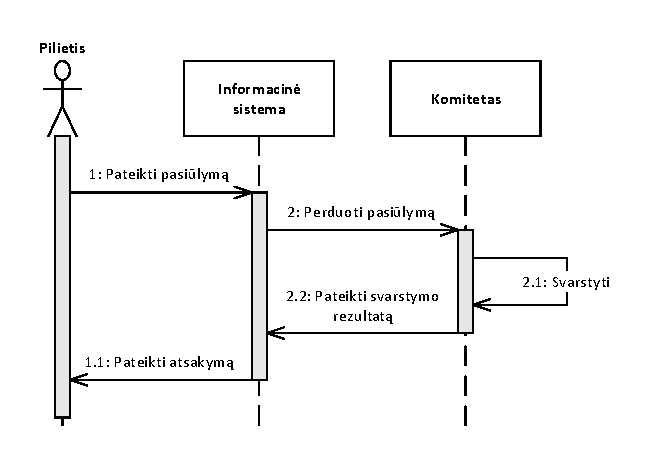
\includegraphics[width=\textwidth]{img/IsPSI1ScenarijausSekuDiagrama3}
			\caption{Naujo pasiūlymo teikimo UML sekų diagrama}
			\label{fig:scenarijusPasiulymoSekuDiagrama}
		\end{figure}
      
		\begin{enumerate}
			\item \underline{Pilietis}, turintis naują idėją varžyboms, \textit{pateikia pasiūlymą} \underline{informacinėje sistemoje}.
			\begin{itemize}
				\item \underline{Informacinė sistema} \underline{piliečiui} \textit{pateikia atsakymą} apie jo pateiktą pasiūlymą.
			\end{itemize}
			\item \underline{Informacinės sistemos} dėka, naujas pasiūlymas \textit{perduodamas} \underline{komitetui}.
			\begin{itemize}
				\item \underline{Komitetas} \textit{svarsto} naują pasiūlymą, t.y. sprendžia, ar pasiūlymą apsimoka įgyvendinti, ar jis atsipirks, patiks žiūrovams bei dalyviams ir pan.
				\item \underline{Komitetas} \textit{pateikia svarstymo rezultatą} \underline{informacinėje sistemoje}.
			\end{itemize}
		\end{enumerate}
      
    \subsubsection*{Organizacijos viduje}
	
	    \begin{figure}[H]
			\centering
			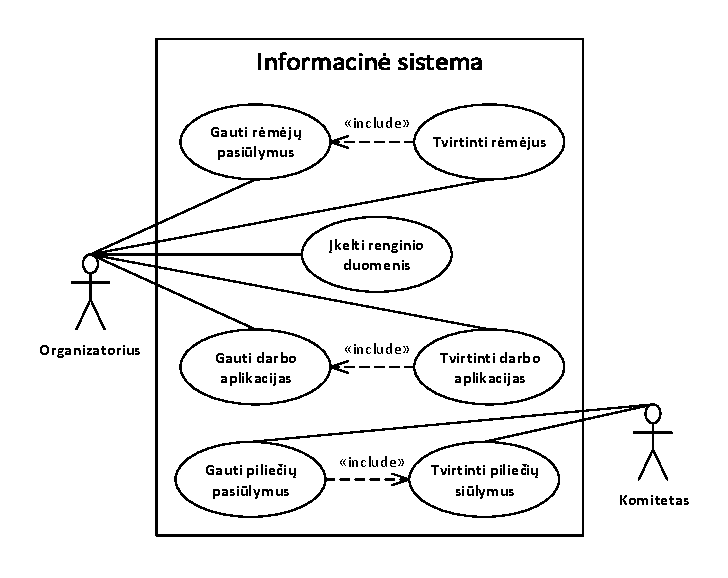
\includegraphics[width=\textwidth]{img/IsPSI1ScenarijausUzduociuDiagrama1}
			\caption{Sistemos teikiamos naudos organizacijos viduje UML užduočių diagrama}
			\label{fig:scenarijusVidausUzduociuDiagrama}
		\end{figure}

		\begin{enumerate}
			\item \underline{Organizatorius}, pasitelkęs informacinę sistemą:
			\begin{itemize}
				\item \textit{Gauna rėmėjų pasiūlymus}. Gavęs juos, \underline{organizatorius} apsvarsto pateiktus pasiūlymus bei  \textit{tvirtina rėmėjus}.
				\item \textit{Įkelia renginio duomenis} į informacinę sistemą.
				\item \textit{Gauna darbo aplikacijas}. Gavęs jas, \underline{organizatorius} apsvarsto bei  \textit{tvirtina darbo aplikacijas} - pateikia teigiamą ar neigiamą atsakymą, priklausomai nuo asmens aplikacijos.
			\end{itemize}
			\item \underline{Komitetas}, pasitelkęs informacinę sistemą:
			\begin{itemize}
				\item \textit{Gauna piliečių pasiūlymus} su naujomis idėjomis varžybų organizavimui. Apsvarstęs juos, \underline{komitetas} \textit{tvirtina piliečių pasiūlymus}.
			\end{itemize}
		\end{enumerate}

    \subsubsection*{Už organizacijos ribų}
	
	    \begin{figure}[H]
			\centering
			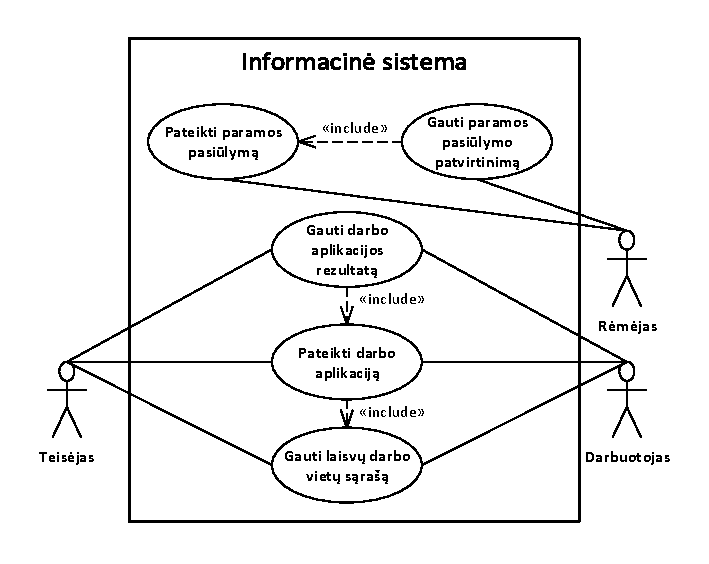
\includegraphics[width=\textwidth]{img/IsPSI1ScenarijausUzduociuDiagrama2}
			\caption{Sistemos išoriniams vykdytojams teikiamos naudos UML užduočių diagrama}
			\label{fig:scenarijusIsoresVykdytojuUzduociuDiagrama}
		\end{figure}

		\begin{enumerate}
			\item \underline{Rėmėjas}, pasitelkęs informacinę sistemą:
			\begin{itemize}
				\item \textit{Pateikia paramos pasiūlymą}. Tuomet \underline{rėmėjas} laukia, kol organizatoriai apsvartys jo išsakytas
					idėjas. Organizatoriams nusprendus priimti paramą, \underline{rėmėjas} \textit{gauna pasiūlymo patvirtinimą}.
			\end{itemize}
			\item \underline{Teisėjas}, pasitelkęs informacinę sistemą:
			\begin{itemize}
				\item \textit{Gauna laisvų} \underline{teisėjo} \textit{darbo vietų sąrašą}. Gavęs sąrašą, \underline{teisėjas}
					\textit{pateikia darbo aplikaciją} informacinėje sistemoje. Organizatoriui apsvarsčius ir nusprendus dėl
					įdarbinimo, \underline{teisėjas} \textit{gauna darbo aplikacijos rezultatą}.
			\end{itemize}
			\item \underline{Darbuotojas}, pasitelkęs informacinę sistemą:
			\begin{itemize}
				\item \textit{Gauna laisvų} įvairaus \textit{pagalbinio darbo vietų sąrašą}. Gavęs sąrašą, pagalbinis \underline{darbuotojas}
					\textit{pateikia darbo aplikaciją} informacinėje sistemoje. Organizatoriui apsvarsčius aplikaciją, \underline{darbuotojas}
					\textit{gauna darbo aplikacijos rezultatą}.
			\end{itemize}
		\end{enumerate}
      
	\subsubsection*{Už organizacijos ribų}
	
		\begin{figure}[H]
			\centering
			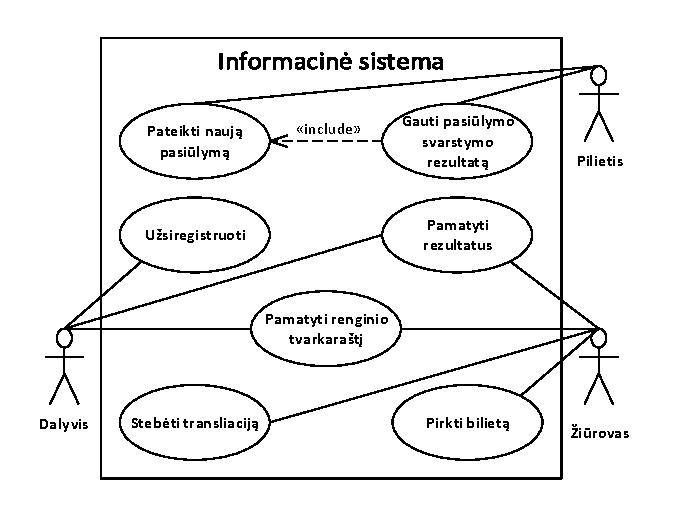
\includegraphics[width=\textwidth]{img/IsPSI1ScenarijausUzduociuDiagrama3}
			\caption{Sistemos išoriniams naudotojams teikiamos naudos UML užduočių diagrama}
			\label{fig:scenarijusIsoresNaudotojuUzduociuDiagrama}
		\end{figure}

		\begin{enumerate}
			\item \underline{Pilietis}, pasitelkęs informacinę sistemą:
			\begin{itemize}
				\item \textit{Pateikia naują pasiūlymą}. Komitetui apsvarsčius \underline{piliečio} pateiktą pasiūlymą, \textit{gauna pasiūlymo svarstymo rezultatą}.
			\end{itemize}
			\item \underline{Dalyvis}, pasitelkęs informacinę sistemą:
			\begin{itemize}
				\item \textit{Užsiregistruoja} į norimas varžybas.
				\item Pasibaigus varžyboms, sistemoje \textit{pamato rezultatus}.
			\end{itemize}
			\item \underline{Žiūrovas}, pasitelkęs informacinę sistemą gali:
			\begin{itemize}
				\item \textit{Pamatyti} būsimų \textit{varžybų renginio tvarkaraštį}.
				\item Pasibaigus varžyboms sistemoje \textit{pamatyti dalyvių rezultatus}.
				\item \textit{Stebėti} tiesioginę ar įrašytą varžybų \textit{transliaciją}.
				\item \textit{Pirkti bilietą} į renginį.
			\end{itemize}
		\end{enumerate}
		
    \section{Struktūrinis programų sistemos modelis} \label{strukturinisPSModelis}
        Šiame modelyje apžvelgiamas sistemos funkcionalumas.
		Žemiau pateikiamos klasių diagramos, atvaizduojančios pagrindines sistemos funkcijas.
		
		\subsection*{Pagrindinių Informacinės Sistemos funkcijų veikla}
		Pirmoje struktūrinio sistemos modelio diagramoje vaizduojama bazinė sistemos veikla.
		Administratorius užtikrina renginių tvarkarašio tikslumą.
		Jis turi galimybę pridėti, pašalinti bei redaguoti kiekvieną renginį.
		Pagal atitinkamą aplinkinių susidomėjimą, administratorius prideda, ištrina ar redaguoja sporto šaką.
		Taip pat, administratorius privalo pridėti ar išimti bilietus į pasirinktą renginį, nurodęs bilietų kainą bei kiekį.
		Pasibaigus varžyboms, administratorius, pasirinkęs dalyvį bei renginį, įveda atitinkamą rezultatą.
		Jei įvestas rezultatas yra klaidingas, administratorius gali jį redaguoti ar ištrinti.
		Administratorius, pasirinkęs renginį, prideda, redaguoja ar ištrina atitinkamą darbuotojo tipą.
		Klasė Renginys neatlieka jokių funkcijų, tačiau savo sudėtyje turi svarbiausias renginio detales, tokias kaip vietos koordinatės, bilietai, ieškomų darbuotojų sąrašas ir kt.
		Vos užsiregistravęs asmuo tampa įprastu vartotoju.
		Vartotojas, norintis gauti papildomų teisių, gali įgauti dalyvio ar darbuotojo poziciją.
		Dalyvis privalo užsiregistruoti į norimą renginį.
		Jei dalyvis nori dalyvauti renginyje, kurio varžybos yra komandinės, jis privalo sukurti komandą, įvesdamas jos pavadinimą bei pridėjęs norimus kitus komandos narius.
		Dalyvis gali ištrinti savo sukurtą komandą.
		Jei dalyvis ar jo komanda nebeketina dalyvauti varžybose, jis gali atšaukti dalyvavimą pasirinkęs atitinkamą renginį.
		Jei dalyvis jau turi savo komandą, tačiau nori į ją pridėti dar vieną narį, jis tai gali padaryti pasirinkęs komandą, į kurią nori pridėti, bei naują komandos narį.
		Pakviestas dalyvis gauna pakvietimą į komandą.
		Apsvarstęs pasiūlymą, jis gali atsakyti į kvietimą jį priimdamas ar atmesdamas.
		Darbuotojo klasėje apibrėžiama konkreti alga bei sąrašas renginių, kuriuose šis asmuo dirba.
		Darbuotojai skirstomi į dvi atskiras grupes - jie gali būti teisėjai bei pagalbiniai darbuotojai.
		Teisėjas, pasibaigus renginiui, pasinaudojęs administratoriaus teisėmis, perduoda rezultatus.
		
		
		\begin{figure}[H]
			\centering
			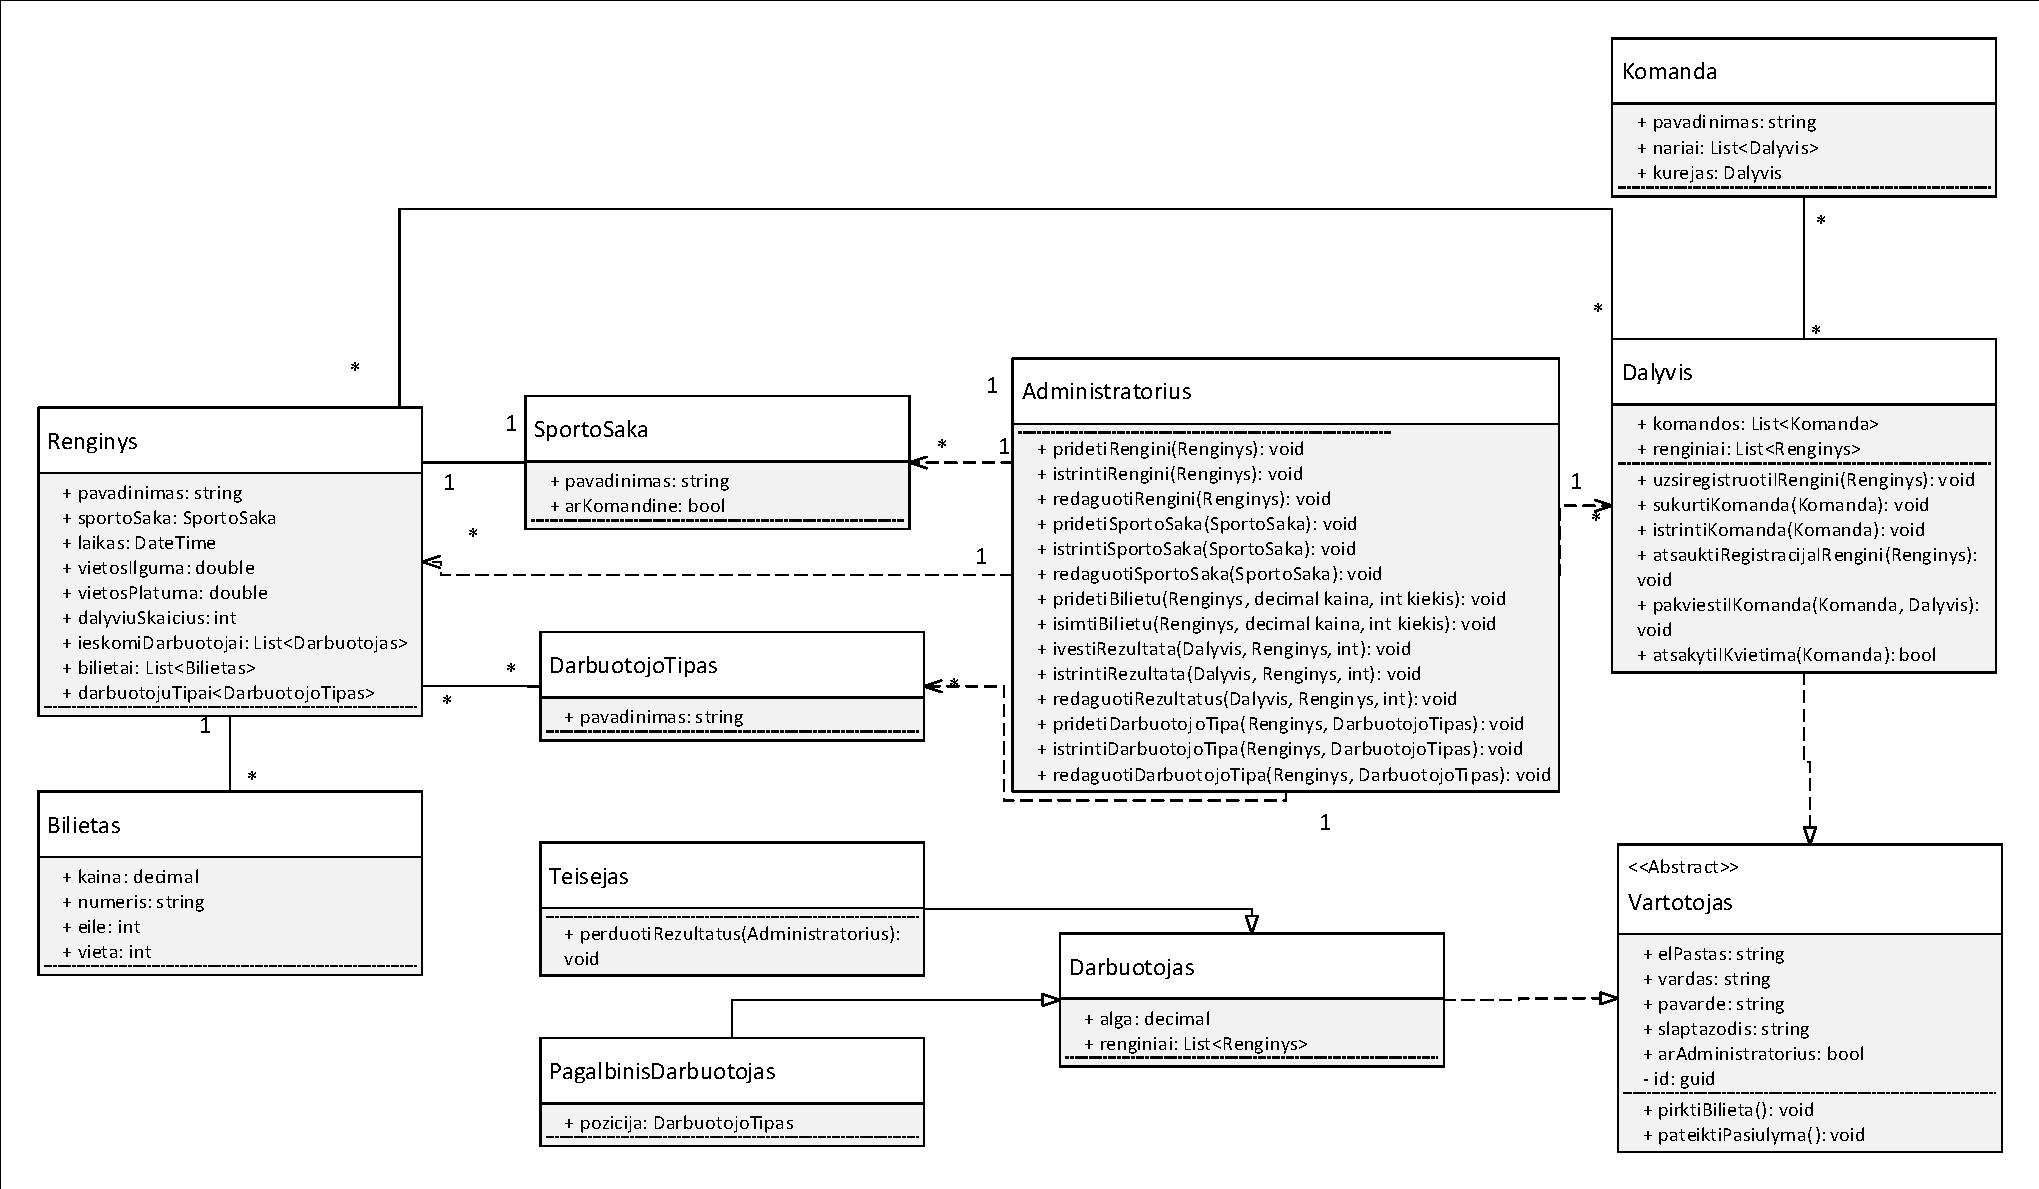
\includegraphics[width=\textwidth]{img/KlasiuDiagrama1}
			\caption{Pagrindinių Informacinės Sistemos funkcijų diagrama}
			\label{fig:PagrindiniuInformacinėsSistemosFunkcijųDiagrama}
		\end{figure}

		\subsection*{Pasiūlymų teikimo posistemės veikla}
		Už naujo pasiūlymo siuntimo funkciją atsakingas pasiūlymų valdiklis, pavaizduotas žemiau esančioje klasių diagramoje.
		Klasės PasiulymuValdiklis vienintelis viešai prieinamas metodas siustiPasiulyma(Pasiulymas) suformatuoja pranešimą ir išsiunčia svarstymo komisijai. Metodo
		grąžintas rezultatas nusako, ar veiksmas pavyko, ar ne. \par
		Pasiūlymų valdiklis priklauso nuo kitos klasės - Pasiulymas. Ji savyje laiko visą informaciją, reikalingą suformuoti pasiūlymo pranešimui - siuntėją bei patį pranešimą.
		Iš siuntėjo išgauti galima tik jo vardą, pavardę bei el. paštą, kad nebūtu galima pakenkti vartotojui ar sugadinti jo informaciją.
		\begin{figure}[H]
			\centering
			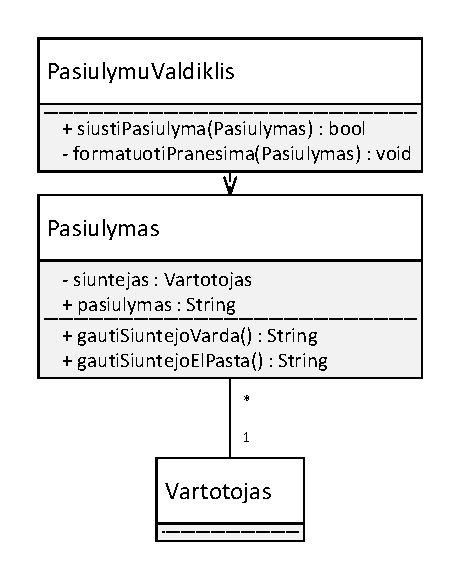
\includegraphics[width=\textwidth, height=10cm, keepaspectratio]{img/KlasiuDiagramaPasiulymai}
			\caption{Pasiūlymų teikimo posistemės klasių diagrama}
			\label{fig:PasiulymuKlasiuDiagrama}
		\end{figure}

		\subsection*{Registracijos posistemės veikla}
		Už įvairias registracijas atsakingas registracijų valdiklis, apibrėžtas klase RegistracijuValdiklis. Jis suteikia galimybę
		užregistruoti darbuotoją (t.y. aplikuoti į tam tikrą darbo vietą), užregistruoti dalyvį į renginį bei užregistruoti visai naują sistemos vartotoją.
		Taip pat klasė turi viešai neprieinamą metodą, skirtą patikrinti, ar vartotojo duomenys yra teisingi. \par
		RegistracijuValdiklis priklauso nuo klasės DarboPasiulymas. Ji savyje laiko nuorodą į renginį, kuriam šis pasiūlymas suteikiamas, bei tame renginyje esančios darbo vietos identifikacinį kodą.
		\begin{figure}[H]
			\centering
			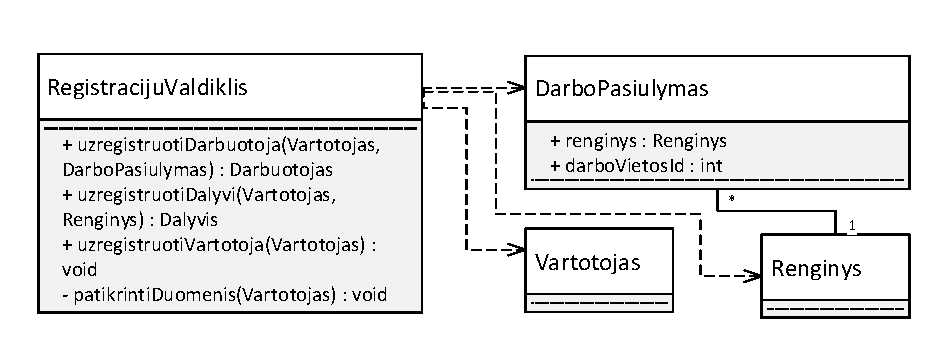
\includegraphics[width=\textwidth]{img/KlasiuDiagramaRegistracija}
			\caption{Registracijos posistemės klasių diagrama}
			\label{fig:RegistracijosKlasiuDiagrama}
		\end{figure}

		\subsection*{Reitingavimo posistemės veikla}
		
		Žemiau pateiktoje klasių diagramoje pateiktas reitingavimo posistemės veikimas.
		Reitingų valdiklis turi metodą gauti vietą. 
		Šis metodas nurodo, kurią vietą varžybose užėmė dalyvis.
		Kitas metodas gauti geriausius dalyvius išrikiuoja dalyvių sąrašą pagal jų pasiektus rezultatus.
		Toliau pateiktas metodas gauti vietą pateiktai komandai grąžina jos užimtą vietą renginyje.
		Veikimas analogiškas gauti dalyvio vietą metodui.
		Paskutinysis metodas gauti geriausias komandas išrikiuoja visas komandas varžybose pagal jų rezultatus.
		
		\begin{figure}[H]
			\centering
			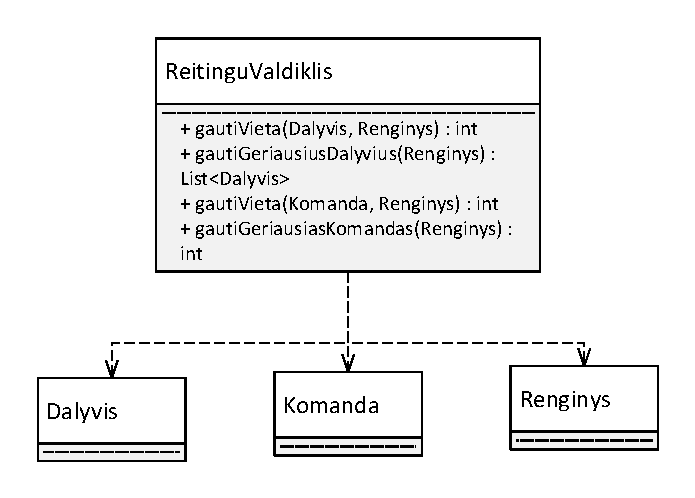
\includegraphics[width=\textwidth]{img/KlasiuDiagramaReitingai}
			\caption{Reitingavimo posistemės klasių diagrama}
			\label{fig:ReitinguKlasiuDiagrama}
		\end{figure}

		\subsection*{Darbo pasiūlymų posistemės veikla}
		Toliau pateiktoje klasių diagramoje vaizduojamas valdiklis, skirtas veiklai su darbo pasiūlymais.
		Jame laikomas privatus laukas - renginys, į kurį ieškomas darbuotojas.
		Šis valdiklis generuoja sąrašą su visais esamais darbo pasiūlymais.
		Darbo pasiūlymų valdiklis darbo vietos id konvertuoja į darbo pasiūlymą.
		
		\begin{figure}[H]
			\centering
			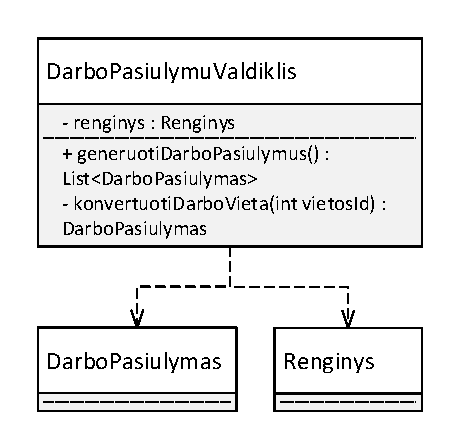
\includegraphics[width=\textwidth, height=10cm, keepaspectratio]{img/KlasiuDiagramaDarboPasiulymai}
			\caption{Darbo pasiūlymų posistemės klasių diagrama}
			\label{fig:DarboPasiulymuDiagrama}
		\end{figure}
		
		\subsection*{Sistemos paketų sąveikos diagrama}
		
		Šioje peketų diagramoje yra pavaizduotos visos aukščiau pateiktos klasės.
		Jos sugrupuotos į paketus, kad aiškiau matytųsi jų tarpusavio sąveika.
		
		\begin{figure}[H]
			\centering
			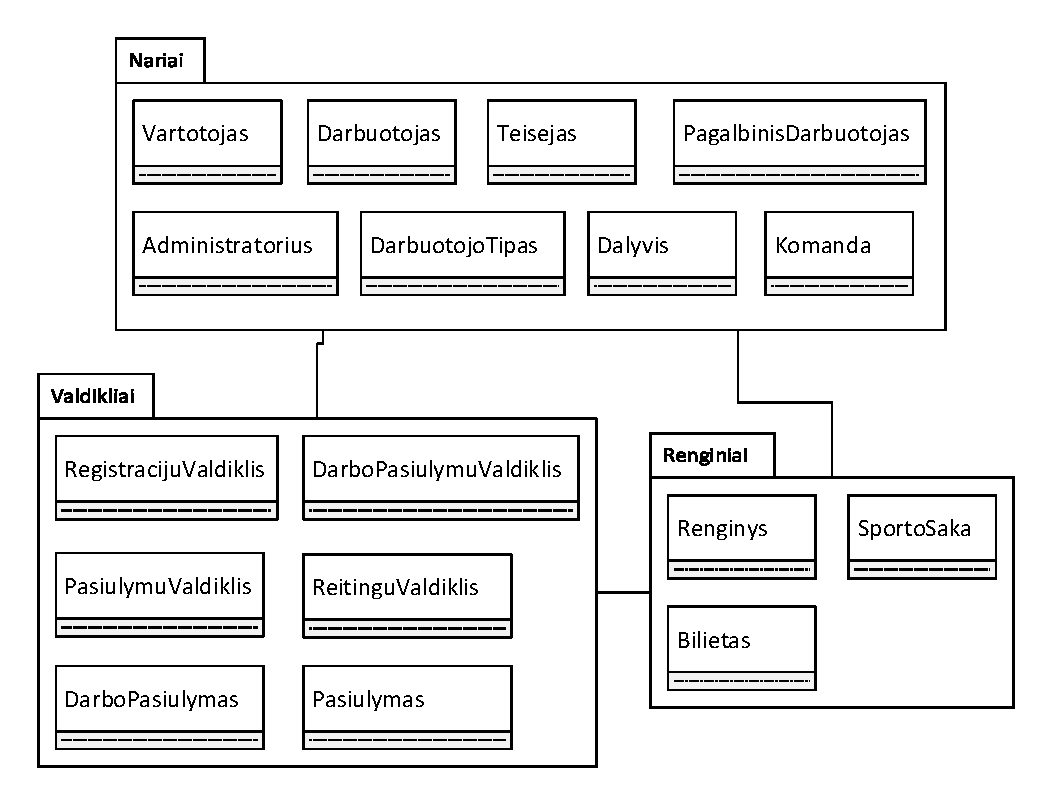
\includegraphics[width=\textwidth]{img/PaketuDiagrama}
			\caption{Sistemos paketų diagrama}
			\label{fig:PaketuDiagrama}
		\end{figure}
		
    \section{Dinaminis programų sistemos modelis} \label{dinaminisPSModelis}
        Šiame modelyje yra apžvelgta, kaip kinta elementų ir informacinės sistemos būsenos programos vykdymo metu. 
		Tai yra atlikta pasitelkiant veiklos ir būsenų UML diagramas.
		Jomis atitinkamai yra aprašomi registracija ir prisijungimas,
		dalyvio registracija į varžybas, teisėjo, norinčio vesti varžybas, registracija, žiūrovo peržiūros.
		\par
		\par
		Apačioje yra pateikta vartotojo registracija ir prisijungimas.
		Norėdamas prisijungti, vartotojas turi užsiregistruoti į sistemą.
		Jeigu jis jau užsiregistravęs, jis iškart gali bandyti prisijungti.
		Tiek registracijos, tiek prisijungimo metu, informacinė sistema patikrina, ar teisingai įvesti duomenys.
		Vartotojui norint atsijungti, sistema įrašo jo sesijos veiklą.
		
		\subsubsection*{Registracija ir prisijungtimas Informacinėje Sistemoje}
		
		\begin{figure}[H]
			\centering
			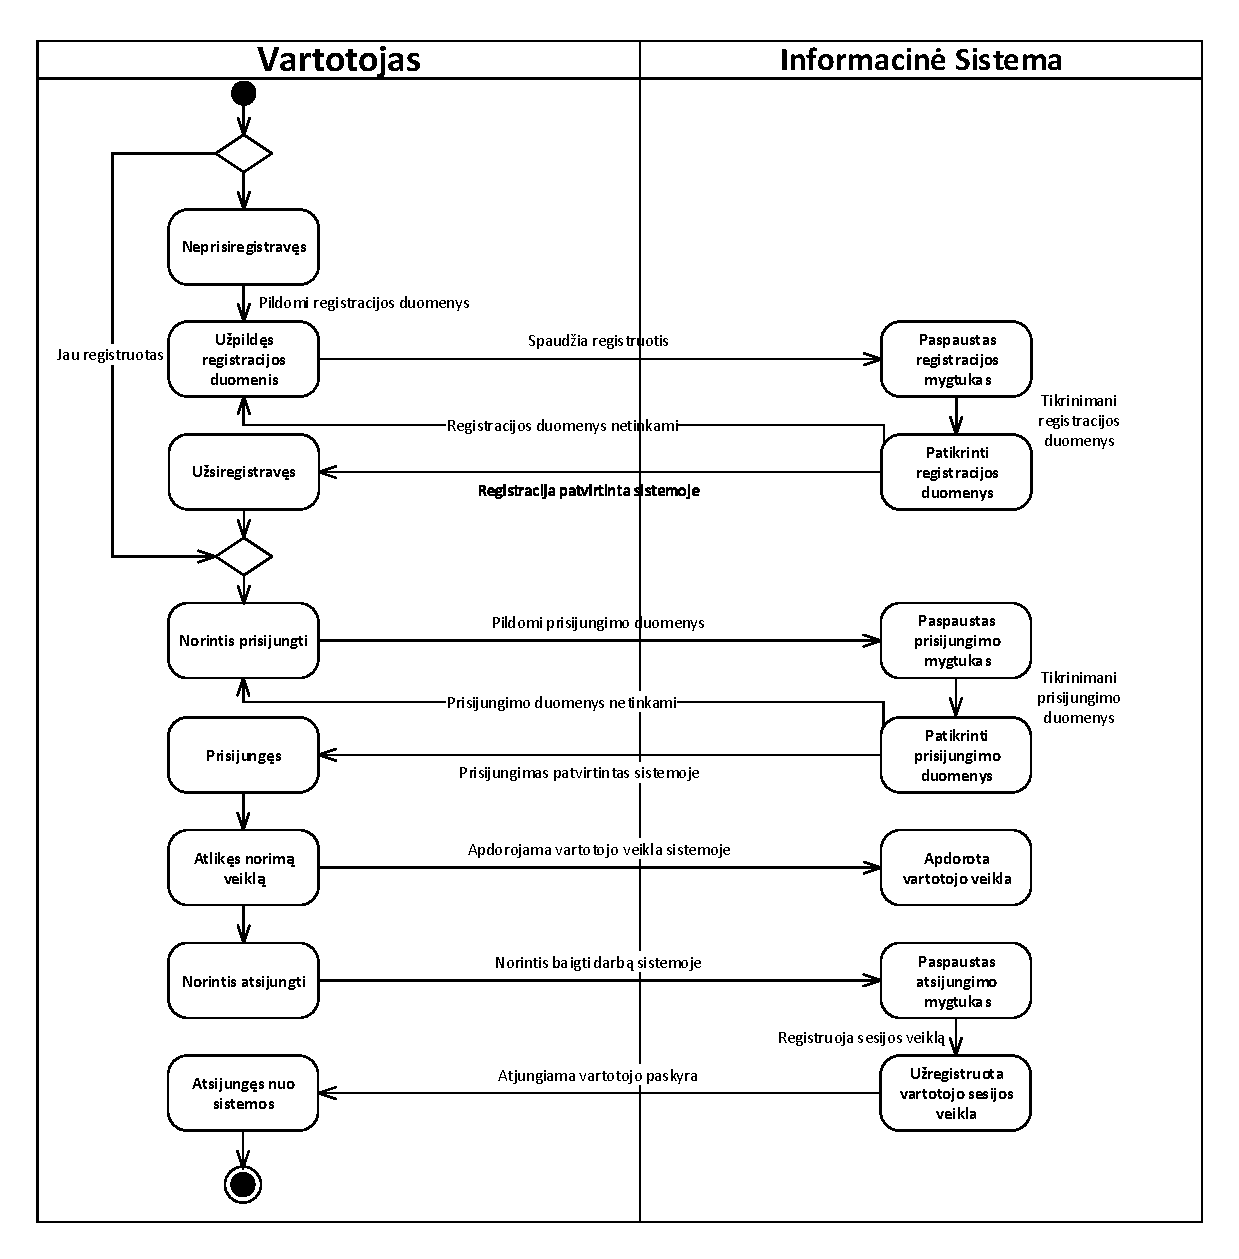
\includegraphics[width=\textwidth]{img/VeiklosDiagrama1}
			\caption{Vartotojo registracijos ir prisijungimo UML veiklos diagrama}
			\label{fig:VartotojoRegistracijosIrPrisijungimoUMLVeiklosDiagrama}
		\end{figure}
		
		Žemiau pateikiama dalyvio registracijos būsenų diagrama. 
		Norėdamas užsiregistruoti, jis užpildo registracijos formą. 
		Sistema patikrina, ar forma atitinka reikalavimus ir dalyvis būna arba atmestas, arba patvirtintas.
		
		\subsubsection*{Dalyvio registracija į varžybas Informacinėje Sistemoje}
		
		\begin{figure}[H]
			\centering
			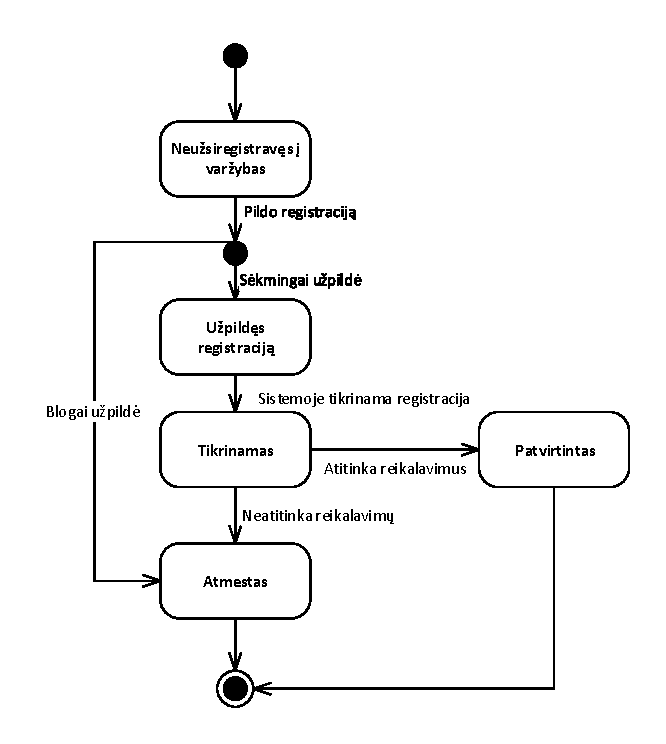
\includegraphics[width=\textwidth]{img/BusenuDiagrama1}
			\caption{Dalyvio registracijos UML busenų diagrama}
			\label{fig:DalyvioRegistracijosUMLBusenuDiagrama}
		\end{figure}
		
		Žemiau pateikiama teisėjo registracijos būsenų diagrama. 
		Norėdamas užsiregistruoti, jis užpildo registracijos formą. 
		Sistema patikrina, ar forma atitinka reikalavimus ir tada teisėjo paraiška būna atmesta arba pateikiama organizatoriui. 
		Organizatorius nusprendžia, ar teisėjas yra tinkamas jo surengtam renginiui.
		
		\subsubsection*{Teisėjo, norinčio vesti varžybas, registracija Informacinėje Sistemoje}
		
		\begin{figure}[H]
			\centering
			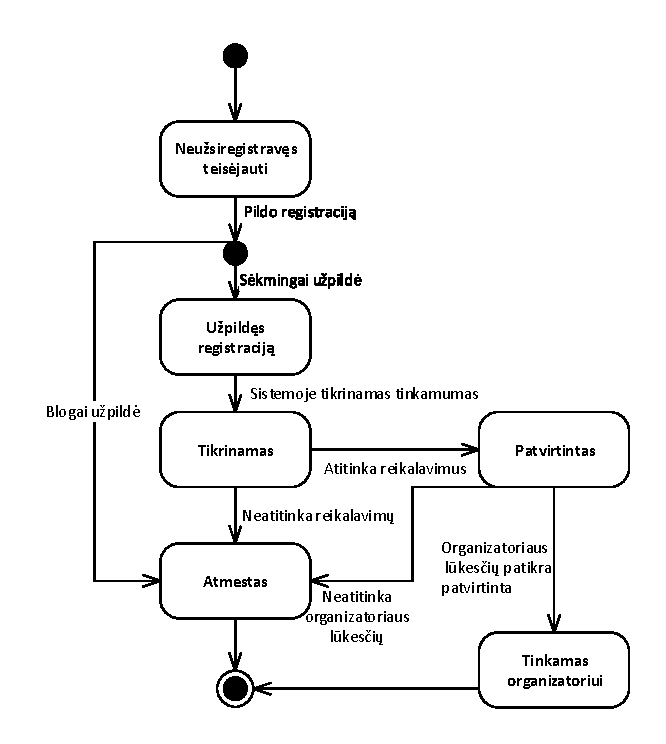
\includegraphics[width=\textwidth]{img/BusenuDiagrama2}
			\caption{Teisėjo registracijos UML busenų diagrama}
			\label{fig:TeisejoRegistracijosUMLBusenuDiagrama}
		\end{figure}
		
		Žemiau pateikiama žiūrovo peržiūrų būsenų diagrama. 
		Žiūrovas yra prisijungęs prie sistemos ir gali peržiūrėti lenteles ar rezultatus jau įvykusių varžybų arba peržiūrėti vaizdo įrašus. 
		Norėdamas peržiūrėti rezultatus jis pasirenka norimas varžybas, vėliau gali pasirinkti ir kitas. 
		Norėdamas peržiūrėti vaizdo įrašus jis turi dvi opcijas - tiesioginę transliaciją arba jau įvykusių varžybų įrašus.
		
		\subsubsection*{Žiūrovo peržiūros Informacinėje Sistemoje}
		
		\begin{figure}[H]
			\centering
			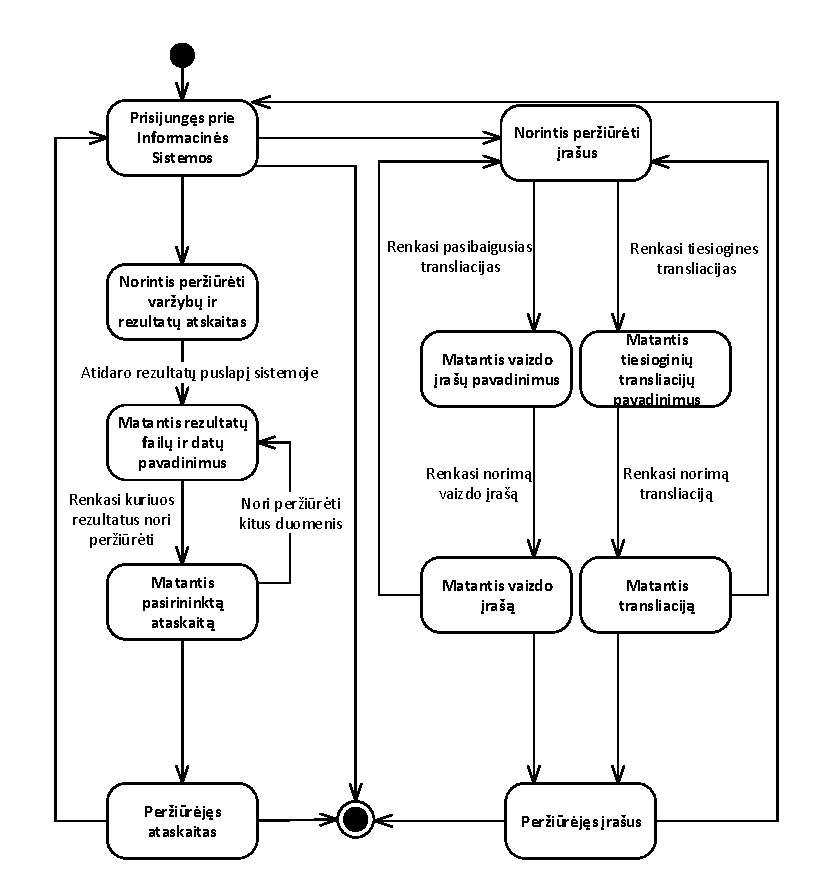
\includegraphics[width=\textwidth]{img/BusenuDiagrama3}
			\caption{Žiūrovo peržiūros UML busenų diagrama}
			\label{fig:ZiurovoPerziurosUMLBusenuDiagrama}
		\end{figure}
		
    \section{Programų sistemos komponentai} \label{PSKomponentai}
        Šiame skyriuje pateikiami pagrindiniai informacinės sistemos komponentų suskirstymai, perteikti komponentų diagramomis.
		Komponentų diagramos išskirstytos į dalis pagal funkcionalumą ir sąsają su informacine sistema.
		Išskirtos svarbiausios sąsajos, tai yra, registracijos ir prisijungimo prie sistemos, registracijos į varžybas, aplikacijos į teisėjavimo darbą bei žiūrovo galimybių.
		\par
		\par
		Žemiau pateikta vartotojo registracijos ir prisijungimo komponentų diagrama.
		Šis komponentas atsakingas už įvestų duomenų tinkamamumą. 
		Yra atskiri registracijos ir prisijungimo autentiškumai. 
		Jie atitinkamai atsakingi už registracijos ir prisijungimo duomenis. 
		Tada duomenys keliauja į informacinę sistemą iš kurios įrašomi į duomenų bazę.

		\begin{figure}[H]
			\centering
			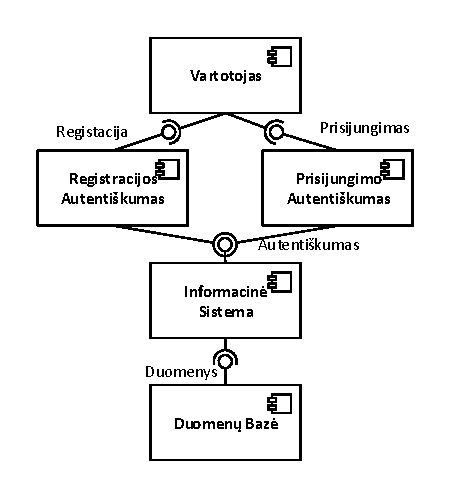
\includegraphics[width=\textwidth, height=10cm, keepaspectratio]{img/KomponentuDiagrama1}
			\caption{Vartotojo registracijos ir prisijungimo UML komponentų diagrama}
			\label{fig:VartotojoRegistracijosIrPrisijungimoUMLKomponentuDiagrama}
		\end{figure}
		
		Žemiau pateikta dalyvio ir komandos registracijos į varžybas komponentų diagrama. 
		Varžybos gali būti tiek individualios, tiek komandinės, todėl yra du komponentai: dalyvis ir komanda. 
		Dalyvis gali įeiti į komandos sudėtį arba dalyvauti individualiose rungtyse. 
		Varžybos siunčia duomenis į informacinę sistemą su dalyvių ir komandų duomenimis. 
		Informacinė sistema įrašo duomenis į duomenų bazę.
		
		\begin{figure}[H]
			\centering
			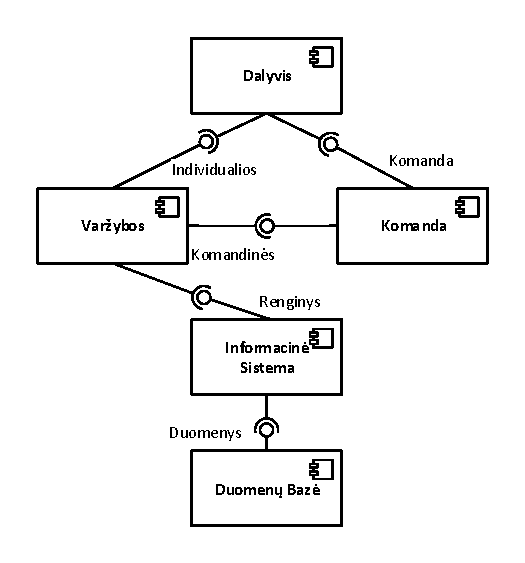
\includegraphics[width=\textwidth, height=10cm, keepaspectratio]{img/KomponentuDiagrama2}
			\caption{Dalyvio ir Komandos registracijos UML komponentų diagrama}
			\label{fig:DalyvioIrKomandosRegistracijosUMLBusenuDiagrama}
		\end{figure}
		
		Žemiau pateikta teisėjo registracijos komponentų diagrama. 
		Teisėjas turi atitikti du reikalavimus, norėdamas teisėjauti renginiui: būti tinkamas organizatoriui ir atitikti sistemos reikavimus. 
		Informacinė sistema gauna duomenis iš teisėjo bei organizatoriaus ir juos įrašo į duomenų bazę. 
		
		\begin{figure}[H]
			\centering
			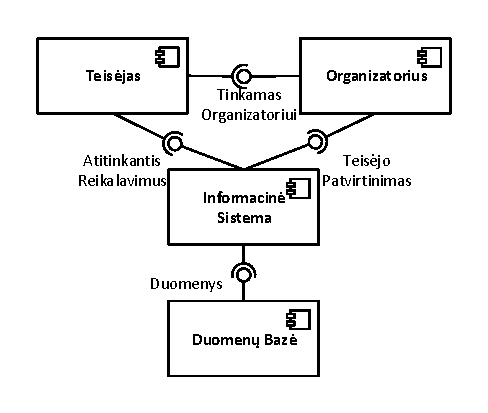
\includegraphics[width=\textwidth, height=10cm, keepaspectratio]{img/KomponentuDiagrama3}
			\caption{Teisėjo registracijos UML komponentų diagrama}
			\label{fig:TeisejoRegistracijosUMLKomponentuDiagrama}
		\end{figure}
		
		Žemiau pateikta žiūrovo peržiūros komponentų diagrama. 
		Žiūrovas turi du pasirinkimus: žiūrėti vaizdo įrašus arba žiūrėti varžybų ataskaitas. 
		Informacinė sistema gauna duomenis iš duomenų bazės. 
		Informacinė sistema suteikia duomenis tiek vaizdo įrašams, tiek varžybų ataskaitoms.
		
		\begin{figure}[H]
			\centering
			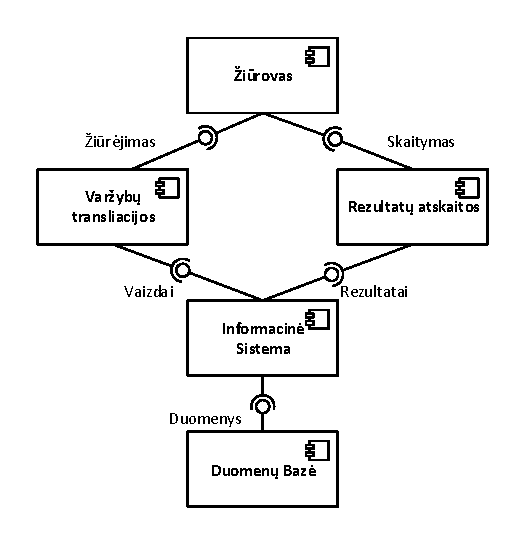
\includegraphics[width=\textwidth, height=10cm, keepaspectratio]{img/KomponentuDiagrama4}
			\caption{Žiūrovo peržiūros UML komponentų diagrama}
			\label{fig:ZiurovoPerziurosUMLKomponentuDiagrama}
		\end{figure}
		
    \section{Komponentų išskirstymas tinkle} \label{komponentuIsskirstymasTinkle}
		
		Diagramoje, pateiktoje apačioje, yra parodyta, kaip tinklapis ir aplikacija bus išdėstyta tinkle.
		Aplikacija veikia iOs, Android ir Windows Phone aplinkose, kurios yra įdiegtos mobiliajame įrenginyje.
		Mobilusis įrenginys, kai yra naudojamasi aplikacija, gali kreiptis į duomenų bazės serverį, kuriame yra MSSQL duomenų bazė.
		Duombazėje yra saugomi visi reikalingi aplikacijos duomenys.
		Personalnis kompiuteris per HTTP protokolą kreipiasi į tinklo serverį, kuriame yra tinklapis.
		Tinklapis, kai prie jo yra prisijungta, gali kreiptis į duomenų bazės serverį, kuriame yra MSSQL duomenų bazė.
		
        \begin{figure}[H]
			\centering
			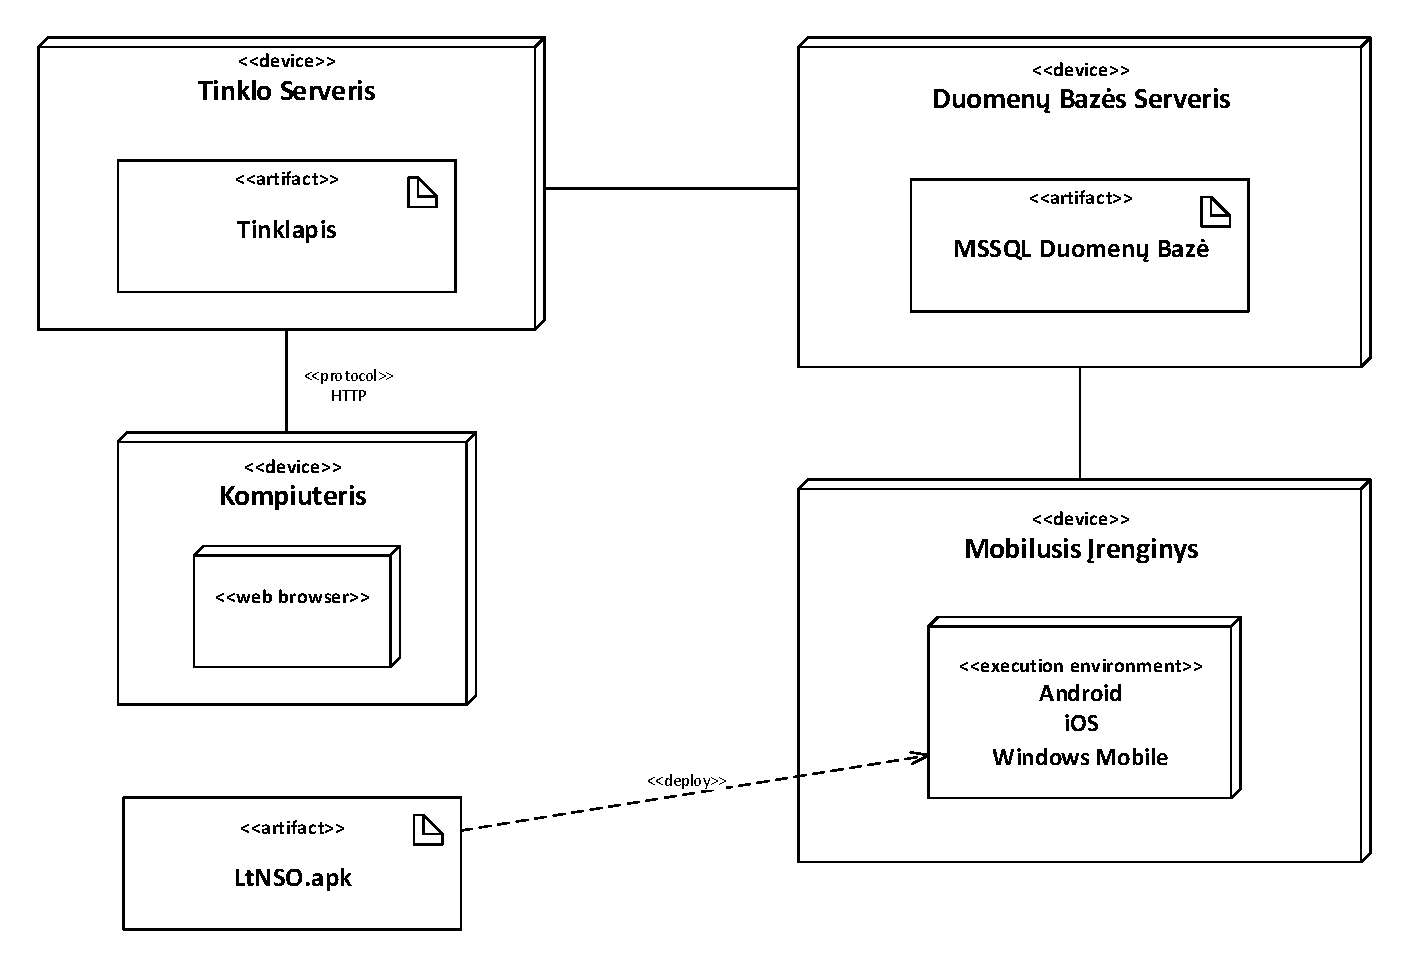
\includegraphics[width=\textwidth]{img/DiegimoDiagrama}
			\caption{UML diegimo diagrama}
			\label{fig:UMLDiegimoDiagrama}
		\end{figure}
		
    \sectionnonum{Literatūros sąrašas} \label{literaturosSarasas}
        \begin{itemize}
			\item Doc. dr. K. Petrausko Programų Sistemų Inžinerijos kurso konspektai
			\item Doc. dr. K. Petrausko Trečiojo laboratorinio darbo struktūra iš: http://www.mif.vu.lt/~karolis/PSI1.html
			\item A. Abran, J. W. Moore, P.Bourque, R. Dupuis, L. L. Tripp - ,,Guide to the Software Engineering Body of Knowledge''
			\item Latex dokumentacija: http://www.latex-project.org/help/documentation/
        \end{itemize}
\end{document}
